\documentclass[twoside,colorbacktitle,accentcolor=tud1b]{tudexercise}
\usepackage[english]{babel}
\usepackage[export]{adjustbox}
%\usepackage{subfig}
\usepackage{subcaption}
\usepackage{paralist}
\usepackage[nolist]{acronym}

\newcommand{\unit}[1]{{\rm\,#1}}
\renewcommand{\labelenumi}{\arabic{enumi}.}


% acronyms
\begin{acronym}
\acro{TM}{Transaction Manager}
\acro{localDB}{local database}
\acro{RM}{Resource Manager}
\acro{JMS}{Java Message Service}
\acro{XA}{X/Open XA}
\end{acronym}

\title{Submission for Milestone 3
\linebreak[1] Middleware Project
\linebreak[1] Winter Term 2014/15}
\subtitle{Pratyush Agnihotri (2387187)\\
Manisha Luthra (2687667) \\
Patrick Welzel (1478819)}

\begin{document}
  \begin{examheader}
    \textmb{Submission for Milestone 3
	\linebreak[1] by: 
      Pratyush Agnihotri (2387187),
      Manisha Luthra (2687667),
      Patrick Welzel (1478819)}
  \end{examheader}
\setcounter{section}{2}
\maketitle

\section*{Global overview}
In this milestone we implemented two main feature categories: Reactive ERP system for shipment tracking via JMS and handling notifications on exceptional events as well as, %publishing and handling events with JMS, 
replication and synchronization of a distributed database.


\section{Message driven shipment tracking and notifications}
In the third and fourth tasks, the shipment tracking need to be done via message technology the Java Message Service (JMS), which triggers the automated shipment updates, position updates and notifications on exceptional events.

\subsection{Architectural overview}
As the employee changes the status of the shipment to "Ready to be shipped" is when the shipments are loaded in some random truck and the reactive mode of the system is activated. To demonstrate the functionality, we have a JMS producer, basically the $PublisherBean$ which is responsible of sending appropriate events. To explicitly handle this, we added a button "Fire events", which then issues command to the $PublisherBean$, which then trigger random events. The $MessageBean$ is then responsible to update the corresponding shipments, saving the events with timestamp in order to display the latest event and sending email to the corresponding customer on the receipt of exception event. The on-the-fly architecture overview of mechanism discussed above for the $Reactive \ ERP \ system$ is illustrated in Figure 1.

\begin{figure}[h!]
  \centering
   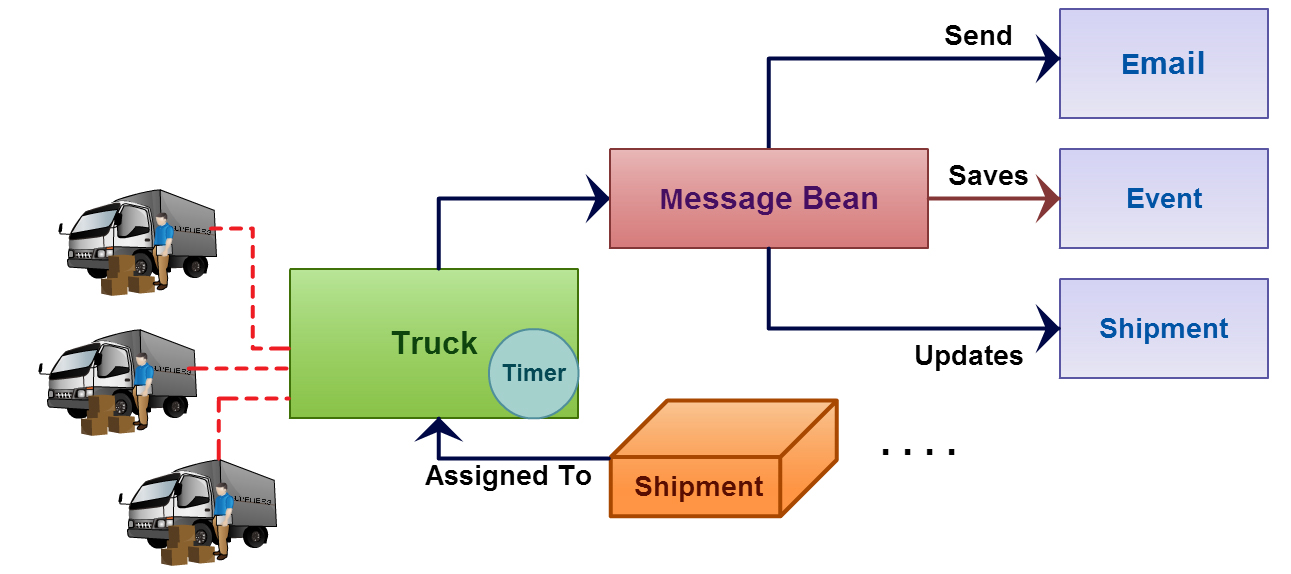
\includegraphics[width=80mm]{TruckMessageBean.jpg}
   \caption{Message driven ERP system}
\end{figure}

\subsection{Implemented features}

\paragraph{Reactive ERP system- Shipment tracking and notifications on exception events}
In the milestone 2, the shipment tracking was only via the employee, when there is an update via employee, the customer could track the change in shipment status. As, new monitoring systems are deployed in the trucks we have integrated a "message driven" shipment update into our system. Now, as there are updates from the truck for the shipments, our "Message-driven bean", would receive the updates and eventually also modify the shipment status on the shipment page. Also, to manage the exceptions such as during a truck accident, an additional check verifies this, and updates the shipment status as well as, triggers the notification to the corresponding customer on his email address. To cope with the requirements of the new monitoring technology, we applied certain changes in the domain model of entities, $Truck$, $Event$ and $Shipment$, that is illustrated in Figure 2.

\begin{figure}[h!]
  \centering
   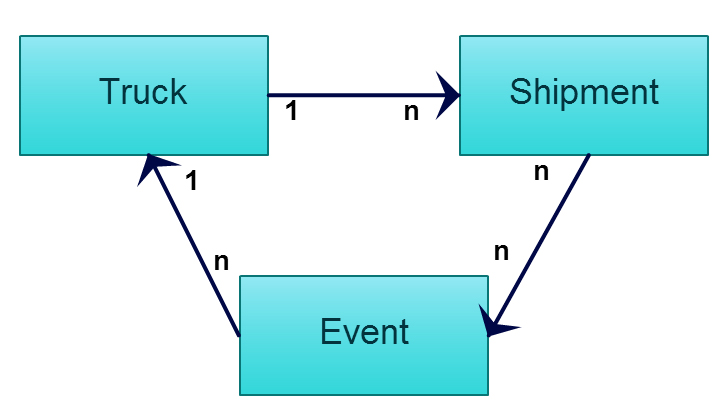
\includegraphics[width=40mm]{EntityRelationShip.jpg}
   \caption{ER-diagram}
\end{figure}

\subsection{Encountered problems/Implementation Alternatives}
\paragraph{Registering JMS resources}
We faced problems with JavaEE in creating the JMS resource and associating with it. JavaEE or NetBeans has problems in associating with the resource on the application server and thus we had to deploy the application again and again in order to solve the problem which was much time-consuming.

\section{Distributed Database}
The fifth and the sixth task were about distributed databases.
In the first part the client should be able to have a local read-only copy of the database in case of connection loss.
The second part was to implement two-phase-commit to synchronize the local database copy.

\subsection{Architectural overview}
On all nodes MySQL is used as the database backend.
All nodes, both the main server and the mobile clients, consist of the web application and a \ac{localDB}.
The mobile clients use a connection proxy to connect either to its local or the remote main database.
The \ac{localDB} will replicate the main servers database with MySQLs \textit{master-slave-replication}\footnote{in MySQL terminology}. The classic architecture of the communication between MySQL master-slave db is illustrated in Figure 3.\footnote{source: https://www.thomas-krenn.com/de/wikiDE/images/0/0c/Mysql-replication.png} and also discussed in the following section as per the representation in Omazon Inc.

\begin{figure}[h!]
  \centering
   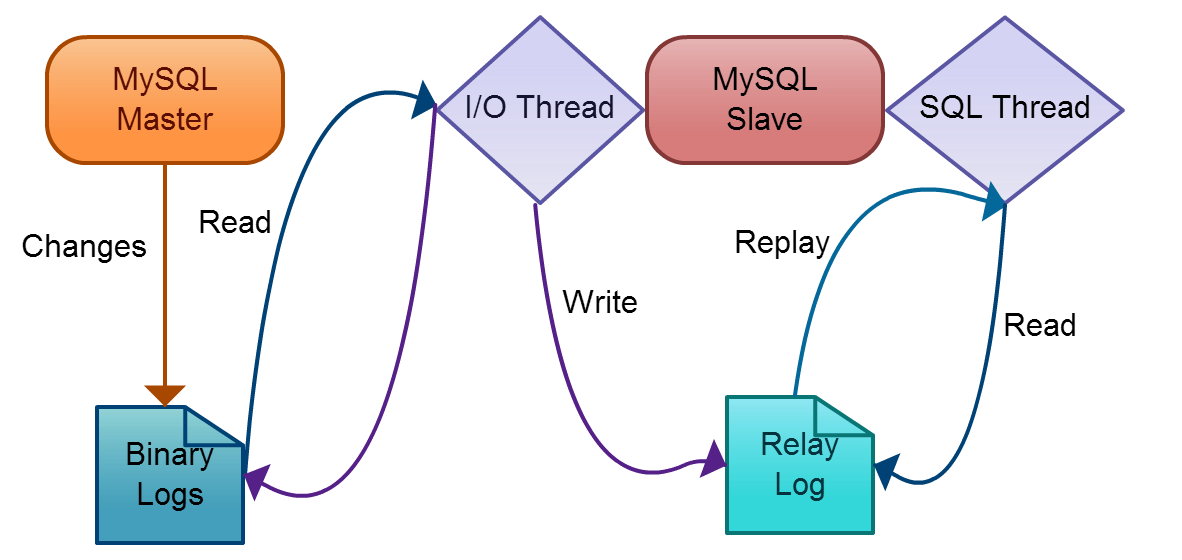
\includegraphics[width=70mm]{MySQLMasterSlave}
   \caption{My SQL master slave communication}
\end{figure}

\subsection{Implemented features}

\paragraph{Online and Offline-mode for mobile clients}
If the mobile client is online, its local database connects to the main database and performs a master-slave replication.
The master will write all changes to a log file that is sent to all connected slaves and replayed there to keep them up to date.
In detail, first the master has to be set up for replication: the bin-log has to be enabled to store the changes\footnote{normally only up to a certain size and for a maximum age; mobile clients falling out of this window have to be bootstrapped with a full database dump} and later send them to the slave replicas and the \textit{REPLICATION} permission has to be granted. 
Then, on a consistent state (e.g. enabling write lock for this step), the current database is saved and copied to the slave.
This would be done when a new mobile client is build, together with assigning it a unique \textit{server ID}.
The client's slave database has to import the database dump and set up to use the master database as replication master (including the info from which point of the log it should start relaying) and finally the slave replication has to be started.
The \ac{localDB} \textbf{only provides read access} to its data, as it is a slave-replicant.
For each database access, the client has to decide if it should use the main database or its local, read-only fallback.
For this all database connections can be given as \textit{connectionUrl} in JDBC connection and the \textit{FailOverReadOnly} property set true. \newpage
This way, the second connection is only used if the first one is unavailable and then only used for read-only mode.
Whether the main database is online or offline, is automatically detected by JDBC and can be fine tuned by several properties, including the connection timeout or the time after which the main server should be checked again. The architectural overview of the aforementioned mobile client architecture in online and offline mode is demonstrated in Figure 4.

\begin{figure}[h!]
  \centering
   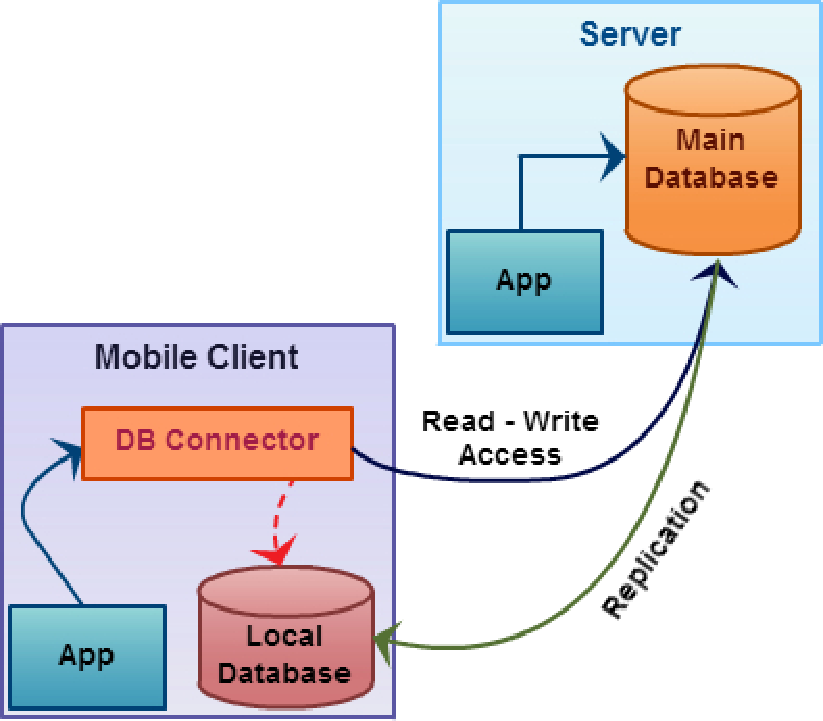
\includegraphics[width=50mm]{ServerMobileClientCommunication}
   \caption{Online and Offline-capable Mobile Client Architecture}
\end{figure}

This usage of MySQL, however would not be advisable in real world scenarios for several reasons: \\
%\begin{enumerate} 
%\itemsep0em 
1. Running a full-blown MySQL server with a full replica of the master database on a mobile client needs many resources probably not available in that environment. \\
2. MySQL replication is not designed over a low-bandwidth unstable mobile connection and may lead to poor performance or interrupted replication. \\
3. Replication is done on the complete database giving full access to the slave which is problematic for sensitive data like personal details. 
%\end{enumerate}

\paragraph{Consistency Guarantee}
The introduced replication method raises the problem of the databases being potentially out of sync for short time periods.
This happens because the main database will allow continuous read and write access while the replication to the local databases is done asynchronously in an best-effort manner ("when there is time").
This can lead to situations where on one application instance, an entity already has updated values while, on another probably a system running under high load still has the old version.

The trivial solution to this is to concentrate both the read and write access to database on the main servers database leaving the local database only providing read-only for offline mode.
As this does not leverages the advantages of distributed database systems regarding load balancing, and the task tells to use two-phase-commit, this has to be improved.

\textbf{Note: At this point it is important to state that we have tried several things but due to problems described below and a lack of time we were not able to get this feature working}, let alone a screen ready version to present. We are describing our approaches nevertheless to document our thoughts and effort put into it.

Based on our existing architecture with MySQL there are the following possible alternatives: \\
%\begin{enumerate}
%\itemsep0em 
1. Using \textbf{MySQL Cluster}, a distributed database setup with multi-node write access using \ac{XA} transactions. \\
2. \textbf{Direct 2PC}: the \ac{TM} of a node connects to all online databases directly, performing 2PC based \ac{XA} transactions. \\
3. \textbf{2PC with in-app \ac{RM}} the \ac{TM} communicates via \ac{JMS} with all online nodes which act as \ac{RM} for \ac{localDB}.
%\end{enumerate}

\paragraph{MySQL Cluster}
MySQL Cluster already implements a synchronized distributed database system.
It consists of Management Nodes, Data Nodes and SQL Nodes; the later to being basically a normal MySQL server split up into the SQL-Capable front end and a data storage back end.
The SQL Nodes also use \ac{XA} transactions while writing transactions to all data nodes.
The mobile client would run both a Data Node and a SQL Node and the main server additionally a Management Node. The configuration overhead and inflexibility in adding and removing nodes rendered this approach too complex and impractical\footnote{even more in practice}.

\paragraph{Direct 2PC}
Another approach would be to use all databases (both the main DB and all locals) directly by each \ac{TM} (being part of the web application).
First all clients and the server have to know about all other running instances and this information has to be kept up to date.
This could be done with \ac{JMS} and a central registry running on the main server.
The \ac{TM} would then open a dedicated connection to each database (the \ac{RM} in this case) resulting in up to $n$ connections on each database and each \ac{TM}.
For coordination of all \ac{RM} during transactions, the \ac{TM} could again use \ac{XA} transactions.
TM tells every branch to prepare themselves to get ready for commit. RM manages and records the actions for the branch in stable storage. These records indicate whether branches are ready to do commit or not. Then, TM starts transactions by sending out transaction request to RMs. If all branches agrees to transaction then RMs answer to TM that they would do the transaction or commit. When TM receives OK from all RMs, it sends out an "OK", do the command, otherwise an "abort", describes basically what a 2PC mechanism does.
%\textbf{TODO: maybe (please discuss if it would help) we should add a SHORT description of xa transactions. not more then 3-4 sentences! Maybe something like: "TM starts transaction by sending out transaction request to RMs. If agreeing to tx, RMs answer to TM that they would do the tx (and thus will reject any tx affecting this txs data as long as tx is pending). When TM receives OK from all RMs, it sends out an \textit{ok, do it} command, otherwise an \textit{abort}"}

Problems could arise in situations where the direct communication between two mobile clients would break but both were still able to communicate with the central server. In these cases the \ac{TM}s on these systems would wait for response from the opposite \ac{RM} indefinitely.
Though, neither of the systems would get kicked out, because they still were able to reach the central system.
This could even lead to system-wide deadlocks when the connection disruption occur after the \ac{RM} agreeing to a commit to the \ac{TM}.
If this agreement or any following command from the \ac{TM} would get lost, the \ac{RM} would block any transaction until it gets a \textit{commit} or \textit{abort} command from the server which will never happen.

\paragraph{2PC with in-app \ac{RM} and JMS}
This approach is quite similar to \textit{Direct 2PC}, but the actual \ac{RM} committing on transactions would be the application itself.
The communication between a \ac{TM} and the \ac{RM}s would be done via JMS and basically be exchanging \ac{XA} transaction objects.
As JMS would use a central message broker, the online/offline state of a database/\ac{RM} would just be determined by the connectivity between its app and the central server.

This approach would be implemented by adding a new $EntityManagerFactory$ that would be responsible for creating $EntityManager$s capable of \ac{XA} transactions via JMS (and act as a message producer in there).
Also, a message driven bean would be needed to listen for incoming transaction requests and responses.
On the main server the message broker would have to be open for communication by all mobile clients.
Joining and leaving nodes would notice the whole swarm by JMS messages and requesting the current set of online nodes on joining.
Periodic ping requests by the main server via JMS would check if all nodes are still online, otherwise removing them from the registry.  An example architecture of the implementation is represented in Figure 5.

\begin{figure}[h!]
  \centering
   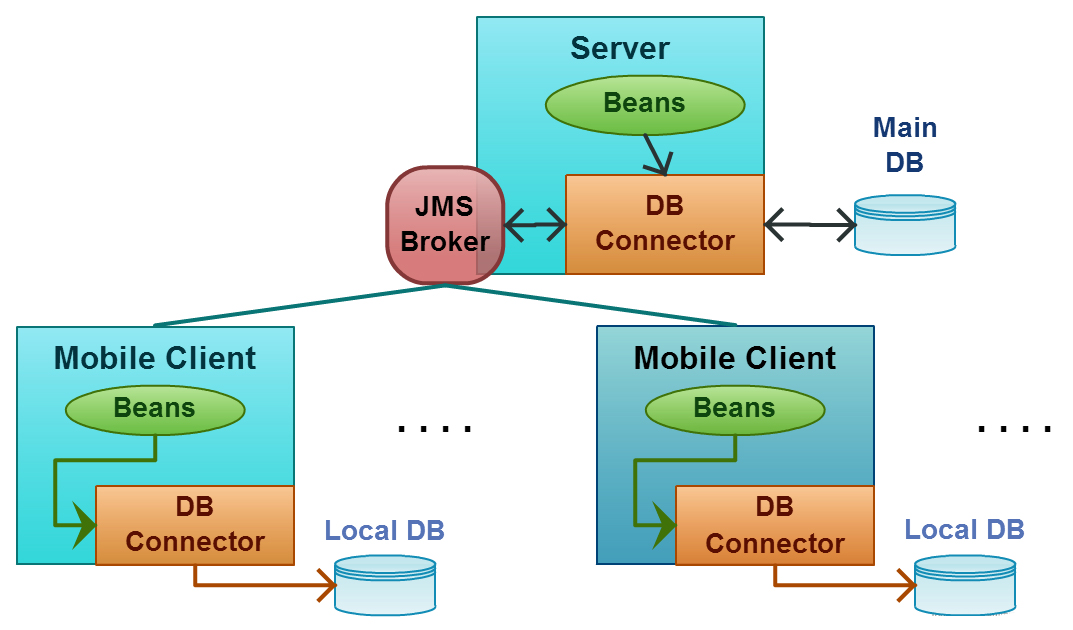
\includegraphics[width=70mm]{2pc}
   \caption{2PC within app}
\end{figure}


\subsection{Encountered problems/Implementation Alternatives}
\paragraph{NetBeans, Glassfish and Persistence}
We had a lot of trouble getting other database connections run with our application, especially the 'drop-and-create' functionality of persistence.
\paragraph{Connecting all the components together}
Due to the first problem and also time contraints we were not able to fully implement the last task i.e \textit{Consistency guarantees} between the various clients. However, we tried to well describe our ideas in the above sections and our understanding of how we could implement the same in Java EE. 
%\textbf{TODO: some more/details explanation of our problems/troubles and probably also why we did not got the last task working/running.}


\end{document}
